%
% $RCSfile: feature_model.tex,v $
%
% Copyright (C) 2002-2008. Christian Heller.
%
% Permission is granted to copy, distribute and/or modify this document
% under the terms of the GNU Free Documentation License, Version 1.1 or
% any later version published by the Free Software Foundation; with no
% Invariant Sections, with no Front-Cover Texts and with no Back-Cover
% Texts. A copy of the license is included in the section entitled
% "GNU Free Documentation License".
%
% http://www.cybop.net
% - Cybernetics Oriented Programming -
%
% http://www.resmedicinae.org
% - Information in Medicine -
%
% Version: $Revision: 1.1 $ $Date: 2008-08-19 20:41:06 $ $Author: christian $
% Authors: Christian Heller <christian.heller@tuxtax.de>
%

\subsubsection{Feature Model}
\label{feature_model_heading}
\index{Feature Model}
\index{Feature Modelling}
\index{System Family}
\index{Software Product Line}
\index{Feature Driven Design}
\index{Software Engineering Process}
\index{SEP}
\index{Feature Oriented Domain Analysis}
\index{FODA}
\index{Traceability}

Czarnecki \cite{czarnecki} sees \emph{Feature Modelling}, a technique for
analysing and capturing \emph{common} and \emph{variable} features of a family
of systems as well as their inter-dependencies in form of a \emph{Feature Model},
as the main contribution of domain engineering to OOA/ OOD methods. The
\emph{System Families}, also called \emph{Software Product Lines}, whose
development feature models shall support, are described by Kai Boellert
\cite{boellert} as \textit{group of software systems that are developed from a
common set of reusable components}. Czarnecki writes:

\begin{quote}
    \emph{Feature Models} represent the configurability aspect of reusable
    software at an abstract level, i.e. without committing to any particular
    implementation technique such as inheritance, aggregation, or parameterized
    classes. Developers construct the initial models of the reusable software
    in the form of feature models and use them to \emph{guide} the design and
    implementation (also called \emph{Feature-driven Design}). To a reuser, on
    the other hand, feature models represent an \emph{overview} of the
    functionality of the reusable software and a guide to \emph{configuring} it
    for a specific usage context.
\end{quote}

\begin{figure}[ht]
    \begin{center}
        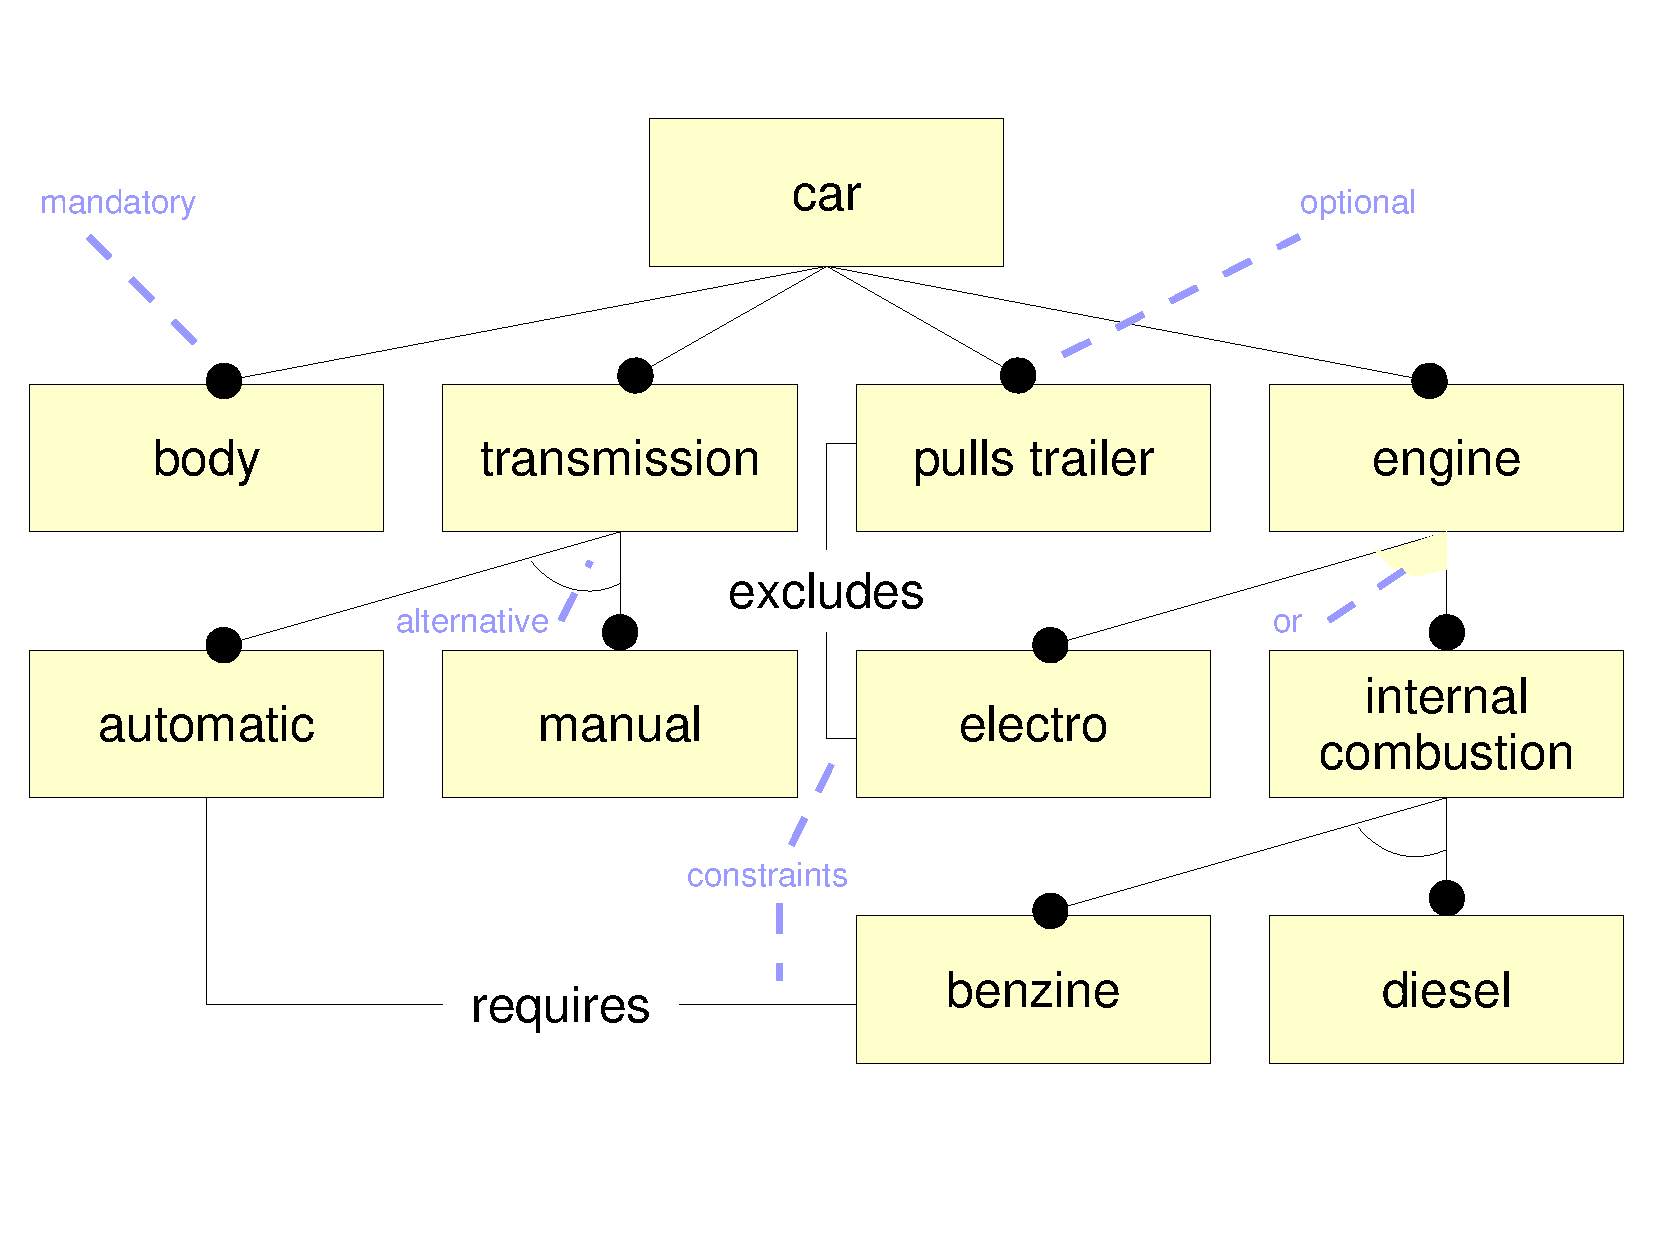
\includegraphics[scale=0.3,angle=-90]{graphic/feature.pdf}
        \caption{Classical Feature Model Diagram of a Car (based on \cite{pashov})}
        \label{feature_figure}
    \end{center}
\end{figure}

In other words, a feature model (figure \ref{feature_figure}) is an additional
form of abstraction within a \emph{Software Engineering Process} (SEP), placed
between analysis- and design models. The properties contained in a feature model
are structured hierarchically. In the \emph{Feature Oriented Domain Analysis}
(FODA) \cite{foda}, a feature model distinguishes three kinds of features:
\emph{Context}, \emph{Representation}, \emph{Operational}. Detlef Streitferdt
\cite{streitferdt200412} defines five feature types:

\begin{enumerate}
    \item \emph{Functional:} used by customer to compose a system
    \item \emph{Interface:} describe required and provided component interfaces
    \item \emph{Parameter:} used to configure functional features
    \item \emph{Structural:} relevant for an automated choice of components
    \item \emph{Conditional:} summarise sub-features to improve readability
\end{enumerate}

Using feature models, the \emph{Traceability} between concrete requirements and
architecture components can be improved. Requirements can better be mapped to
architecture elements, so that also the \emph{Communication} between
stakeholders in the development process can profit. The big abstraction gap
(number \emph{1} in figure \ref{gaps_figure} of section
\ref{abstraction_gaps_heading}) gets split into two smaller (\emph{1a} and
\emph{1b} in figure \ref{gaps_figure}) that do not close the gap conclusively,
but make it easier to cross. The disadvantage of using feature models in a SEP,
however, is that another abstraction gap causing additional effort is created
through them.

The knowledge schema and language introduced in chapters
\ref{knowledge_schema_heading} and \ref{cybernetics_oriented_language_heading}
use a hierarchical structure comparable to the feature model. Their elements,
though, do belong to just one of two possible kinds: \emph{whole-part} model or
\emph{meta property} model. CYBOP knowledge models merge \emph{some} of the
information that would traditionally be found in feature models with that
contained in the design diagrams and might thus be able to eliminate gap 1b.
Non-functional requirements like \emph{Performance}, \emph{Scalability},
\emph{Usability} or \emph{Memory Efficiency} are \emph{not} part of a CYBOP
knowledge model, since they have nothing to do with the actual modelling of
real-world items in form of abstract concepts and belong into a corresponding
analysis- and specification document only.
